\documentclass[12pt,twoside]{article}
\usepackage[noae]{Sweave}
\usepackage{caxetexFree}
\usepackage{lipsum}
\usepackage{titlesec}
\usepackage{bm}
\titleformat{\paragraph}[runin]{\normalfont\normalsize\textsb}{\theparagraph}{1em}{}
\newcommand{\myTitle}{Judicial methods masterclass}
\title{\myTitle}
\author{Chris Hanretty}
\date{May 2016}
\newcommand{\chaptermark}

%% From https://github.com/minrk/ipython/commit/325e76d80861d5cec65b08396c39c6316cde0912

    % commands and environments needed by pandoc snippets
    % extracted from the output of `pandoc -s`
    
    \DefineShortVerb[commandchars=\\\{\}]{\|}
    \DefineVerbatimEnvironment{Highlighting}{Verbatim}{commandchars=\\\{\}}
    % Add ',fontsize=\small' for more characters per line
    \newenvironment{Shaded}{}{}
    \newcommand{\KeywordTok}[1]{\textcolor[rgb]{0.00,0.44,0.13}{\textbf{{#1}}}}
    \newcommand{\DataTypeTok}[1]{\textcolor[rgb]{0.56,0.13,0.00}{{#1}}}
    \newcommand{\DecValTok}[1]{\textcolor[rgb]{0.25,0.63,0.44}{{#1}}}
    \newcommand{\BaseNTok}[1]{\textcolor[rgb]{0.25,0.63,0.44}{{#1}}}
    \newcommand{\FloatTok}[1]{\textcolor[rgb]{0.25,0.63,0.44}{{#1}}}
    \newcommand{\CharTok}[1]{\textcolor[rgb]{0.25,0.44,0.63}{{#1}}}
    \newcommand{\StringTok}[1]{\textcolor[rgb]{0.25,0.44,0.63}{{#1}}}
    \newcommand{\CommentTok}[1]{\textcolor[rgb]{0.38,0.63,0.69}{\textit{{#1}}}}
    \newcommand{\OtherTok}[1]{\textcolor[rgb]{0.00,0.44,0.13}{{#1}}}
    \newcommand{\AlertTok}[1]{\textcolor[rgb]{1.00,0.00,0.00}{\textbf{{#1}}}}
    \newcommand{\FunctionTok}[1]{\textcolor[rgb]{0.02,0.16,0.49}{{#1}}}
    \newcommand{\RegionMarkerTok}[1]{{#1}}
    \newcommand{\ErrorTok}[1]{\textcolor[rgb]{1.00,0.00,0.00}{\textbf{{#1}}}}
    \newcommand{\NormalTok}[1]{{#1}}
\providecommand{\tightlist}{%
  \setlength{\itemsep}{0pt}\setlength{\parskip}{0pt}}    
\pagestyle{fancy}
\renewcommand{\chaptermark}[1]{\markboth{#1}{}}
\fancyhead{} % clear all header fields
\fancyhead[CE]{\rightmark}
\fancyhead[CO]{\leftmark}
\fancyfoot{} % clear all footer fields
\fancyfootoffset[RO]{-0.25in}
\fancyfootoffset[LE]{-0.25in}
\fancyfootoffset[RE]{-0.25in}
\fancyfootoffset[LO]{-0.25in}
\fancyfoot[RO]{\thepage}
\fancyfoot[LE]{\thepage}
\fancyfoot[RE]{\texttt{\jobname{}.tex}, \textsf{revised \today}}
\fancyfoot[LO]{\texttt{\jobname{}.tex}, \textsf{revised \today}}

\renewcommand{\headrulewidth}{0pt}  %1.4

\setlength{\footskip}{33pt}

% Create headerless version for "plain" pages, 
% e.g., page 1 of a paper
\fancypagestyle{plain}{%
\fancyhf{} % clear all header and footer fields
\fancyfootoffset[RO]{-0.25in}
\fancyfootoffset[LE]{-0.25in}
\fancyfootoffset[RE]{-0.25in}
\fancyfootoffset[LO]{-0.25in}
\fancyfoot[RO]{\thepage}
\fancyfoot[LE]{\thepage}
\fancyfoot[RE]{\texttt{\jobname{}.tex}, \textsf{revised \today}}
\fancyfoot[LO]{\texttt{\jobname{}.tex}, \textsf{revised \today}}
\renewcommand{\headrulewidth}{0pt}
\renewcommand{\footrulewidth}{0pt}}

 \renewcommand{\leftmark}{\textsc{\caps{chris hanretty}}~~\(\cdot\)~~\emph{\textsb{%
\myTitle{}%
}}}
 \renewcommand{\rightmark}{\textsc{\caps{chris hanretty}}~~\(\cdot\)~~\emph{\textsb{%
\myTitle{}%
}}}



\begin{document}
\maketitle

\section{Introduction}\label{introduction}

\subsection{About myself}\label{about-myself}

I'll begin by saying something about myself. I'm a Reader in Politics at
the University of East Anglia. I do research on two main areas:
political representation, and judicial behaviour. I've previously
published on judicial behaviour in the UK and in continental Europe.

I am \emph{not} a lawyer. I've not done a degree in law. I've had to
learn about the law, but I've done so in an unstructured way. And so,
many of the things that I say may be legally naïve. Of course, that may
be because the models I describe are legally naïve.

\subsection{About you}\label{about-you}

That's me. What about you?

I'm going to assume that you are all lawyers who are interested in
empirical methods. But I'm not going to assume that you have any
knowledge of statistics.

I don't know whether you want to use empirical methods, or consume
empirical methods. But I'll teach you how I would use these methods of
analysis. That way I hope you'll get a better understanding of how to
interpret these kinds of methods when you encounter them.

Some of you, of course, may already have a good knowledge of statistics.
You may find the first part of this masterclass a little too basic. I
can only apologise, and hope that you find certain parts to be a useful
refresher.

\subsection{About the course}\label{about-the-course}

The first half of this course deals with decision-making by individual
judges. I'll look first at the simple case where a judge has to make a
continuous decision. That will be our way of looking at simple linear
regression.

I'll then move on to the case where a judge has to make a binary
decision. That allows us to look at logistic regression. Logistic
regression will then stay with us throughout the course.

I'll then progressively introduce certain complications. These
complications will result from introducing multiple judges, and from
introducing situations where judges are not randomly assigned to cases.

That first half of the course will be looking at variation across cases.
But there's another kind of variation that's interesting. That's
variation within a single case, which arises because judges disagree.
And so in the second half of the course I'll look at methods for the
analysis of dissent.

In particular, I'll look at what are called item response models. Like
logistic regression models, we're trying to explain a binary outcome.
Either the judge did or didn't dissent. But these models are more
complicated than logistic regression models. The meaning of dissent
changes over cases. Sometimes dissent might be ``liberal''. Sometimes
dissent might be ``conservative''. Item response models help us to
figure out which it is, by looking at the patterns of dissent.

As I go, I'll try to give published examples which have used these
techniques. I'll also try to provide code that will replicate these
results. I use statistics software called R. Many of the things that we
do in the first half of the course can be done in any statistics
package. They can be done in SPSS, or Stata, or even Excel if you're
masochistic enough. But many of the things we do in the second half of
the course can best be done in R.

\section{Random assignment, single judge, continuous
outcome}\label{random-assignment-single-judge-continuous-outcome}

I'm going to start with the simplest possible example. That's the case
where

\begin{itemize}
\tightlist
\item
  a single judge is randomly assigned to a case, and
\item
  must make a continuous, numeric, decision.
\end{itemize}

There are two common situations where judges must make continuous
numeric decisions. The first is when judges make financial awards for
damages. In this case, the decision is the amount of money, whether
that's one, ten, or a hundred thousand euros. The second situation is
when judges send people to prison. In this case, the decision is the
length of the criminal sentence, whether that's ten, a hundred, or a
thousand days.

I start with these continuous decisions because they're easy to model.
Specifically, we can model them using linear regression. The intuition
behind linear regression is easy to understand. You see it every time
you see a scatter-plot.

Here's a very famous scatter-plot. It comes from the 19th century
sociologist Francis Galton. On the horizontal axis, we have the height
of parents. On the vertical axis, we have the height of children.

\begin{figure}[htbp]
\centering
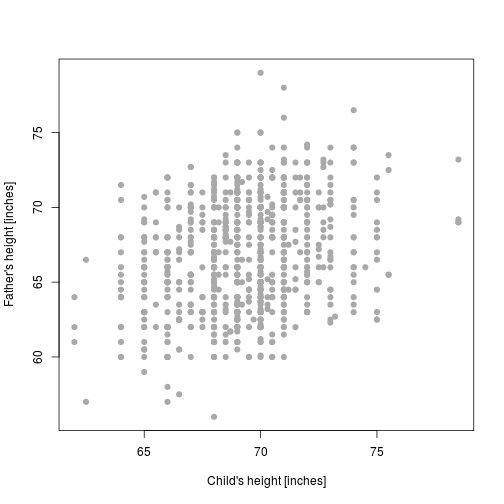
\includegraphics{figure/galton-1.png}
\caption{Galton's height data}
\end{figure}

You can see there's a relationship there. The taller the parents, the
taller the children, on average.

\begin{figure}[htbp]
\centering
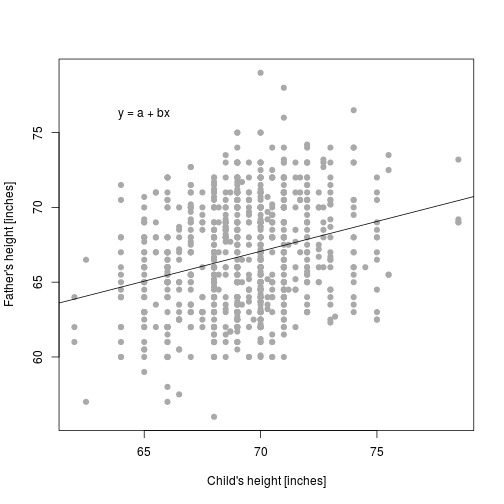
\includegraphics{figure/galton2-1.png}
\caption{Galton's height data}
\end{figure}

\begin{figure}[htbp]
\centering
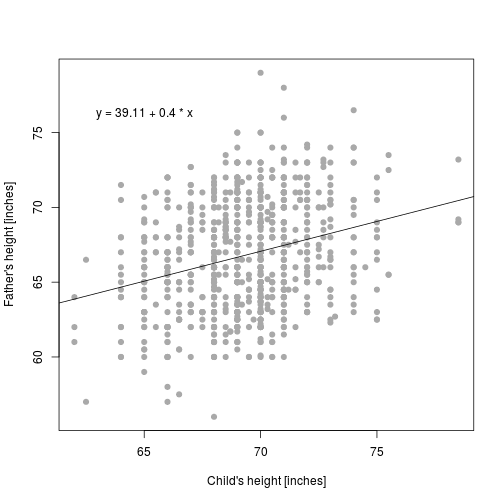
\includegraphics{figure/galton3-1.png}
\caption{Galton's height data}
\end{figure}

We can summarize that relationship using an equation. That's the
equation for the straight line: \(y = a + bx\). I'm going to refer to
the \(a\) as the intercept, and \(b\) as a coefficient.

There are lots of different possible values for a and b. But the
best-fitting values are here: \(a = 39.11\) and \(b = 0.4\). What does
that \(b\) mean?

It means that for every extra inch in parental height, child height goes
up by 0.4. Formally: for every single unit change in x, the dependent
variable changes by b.

How can we use that to examine the impact of judges? This equation is a
way of connecting two numbers -- but judges aren't numbers.

Well, we can turn judges into numbers. Let's imagine a situation with
two judges: Judge Soft and Judge Hard. And suppose Judges Soft and Hard
take the following decisions in sentencing.

I'm going to create what's known as dummy variable. That's a variable
which has a value either of zero or a value of one. That dummy variable
is going to have a value of one when judge Hard decides a case. It'll
have a value of zero when judge Soft decides a case. To use another term
of art: that means that judge Soft is our ``reference level'', or
``reference category''.

We can the create another graph. Here we have the value of the dummy
variable on the horizontal axis. We have the length of the sentence on
the vertical axis.

\begin{figure}[htbp]
\centering
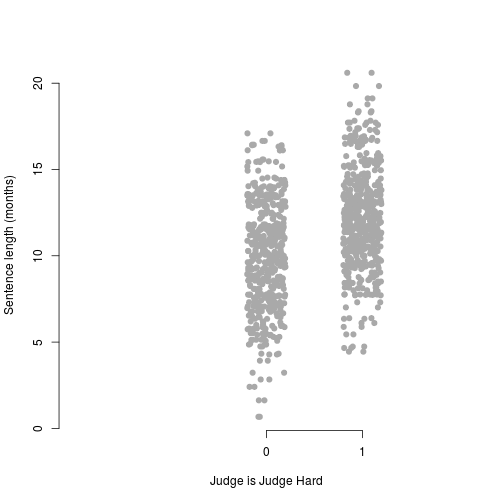
\includegraphics{figure/fakeplot-1.png}
\caption{Plot of a sentencing outcome}
\end{figure}

Just as before, we can draw the best-fitting line through those points.
And that equation looks a little bit like this.

Here, the value of \(b\) is 2.21. That just means that when the value of
the Hard dummy variable is 1, sentence lengths are 2.21 units higher.
Alternately, when judge Hard is hearing the case, sentence lengths are
2.21 units longer than when Judge Soft is hearing the case.

We could have done this differently. We could have chosen Judge Hard as
the reference level. Does anyone know what the value of \(b\) would have
been then? The choice of reference level is entirely arbitrary.

Linear regression thus enables us to make claims like, ``compared to a
reference judge, judge X imposes sentences that are ? months longer''.
We know that this difference must be due to the judge. It can't be due
to the types of cases that Judges Soft and Hard hear. If Judge Hard
systematically heard cases which deserved longer sentences, then the
assignment of cases to judges wouldn't really be random, would it?

If we had information on all the cases heard by judges Soft and Hard, we
could stop there. But very often, we only have information on a sample
of cases. In those circumstances, we may want to know -- are the
differences which we identify in our sample of cases also likely to be
found in the full population of cases heard by these two judges.

That's when the whole machinery of statistical significance testing
comes in. I'll not discuss the details of this here. I'll just show you
what it looks like in R.

You've already seen the first few lines of the data.

\begin{verbatim}
##   Judge  Sentence JudgeHard
## 1  Hard 16.595639         1
## 2  Soft 13.580389         0
## 3  Hard 12.178373         1
## 4  Soft  4.746378         0
## 5  Hard 15.378565         1
## 6  Soft 10.644786         0
\end{verbatim}

Here's the code that generates the regression model.

\begin{Shaded}
\begin{Highlighting}[]
\NormalTok{mod <-}\StringTok{ }\KeywordTok{lm}\NormalTok{(Sentence ~}\StringTok{ }\NormalTok{JudgeHard, }\DataTypeTok{data =} \NormalTok{dat)}
\end{Highlighting}
\end{Shaded}

Here's the R output.

\begin{verbatim}
## 
## Call:
## lm(formula = Sentence ~ JudgeHard, data = dat)
## 
## Residuals:
##     Min      1Q  Median      3Q     Max 
## -9.2178 -2.1174 -0.0311  1.9267  8.5047 
## 
## Coefficients:
##             Estimate Std. Error t value Pr(>|t|)    
## (Intercept)   9.8885     0.1343   73.61   <2e-16 ***
## JudgeHard     2.2093     0.1900   11.63   <2e-16 ***
## ---
## Signif. codes:  0 '***' 0.001 '**' 0.01 '*' 0.05 '.' 0.1 ' ' 1
## 
## Residual standard error: 3.004 on 998 degrees of freedom
## Multiple R-squared:  0.1193, Adjusted R-squared:  0.1184 
## F-statistic: 135.2 on 1 and 998 DF,  p-value: < 2.2e-16
\end{verbatim}

And here's what you would see in a published journal article.

\begin{verbatim}
## Error in dimnames(x$coefficients)[[3]]: subscript out of bounds
\end{verbatim}

\begin{verbatim}
## Error in if (tail(stdout, 1) == "") {: argument is of length zero
\end{verbatim}

You can see the same value of \(b\) as before. But now there's a second
number below it. That's the standard error associated with our estimate
of \(b\). If the standard error is very small compared to the estimate,
then we accept that there's probably a real effect there. In particular,
we would be confident that Judge Hard was harsher if the estimate was
two times the standard error.

We could extend this model in a number of different ways.

First, we could add additional control variables. We don't need these
control variables. If we really have random assignment of judges to
cases, then these control variables won't affect our estimate, \(b\).
But these control variables will make our estimate more precise. They'll
cause the standard error around our estimate to shrink as we add in more
information.

Second, we could add additional judges. Adding additional judges is
easy. We just create a new dummy variable for each of them. Very often
our statistical software will do this for us. Generally, with N judges,
we'll end up creating N-1 dummy variables.

Third, we could transform our dependent variable. Sometimes, regression
models make impossible predictions. Think back to the equation from the
Galton data. If we had carried that line back far enough, we could have
made a prediction that someone would have negative height. That's not
possible. Sometimes, researchers deal with this problem by taking the
natural log of their data, and modelling that natural log. The natural
log takes positive values and maps them into an unrestricted space. You
can then make predictions about natural logs that make sense when
they're transformed back on to the original scale.

The problem with this is that these models are slightly harder to
interpret. Here's a model using the same data as above, but now the
sentence length is log transformed.

\begin{verbatim}
## Error in dimnames(x$coefficients)[[3]]: subscript out of bounds
\end{verbatim}

\begin{verbatim}
## Error in if (tail(stdout, 1) == "") {: argument is of length zero
\end{verbatim}

How can we interpret this? In this instance, the coefficient is 0.23.
What does that mean? It means that when this judge is deciding the case,
sentences are exp(0.23) percent longer. And we can go back to the
original model to check that this is the case.

\section{Random assignment, single judge, dichotomous
outcome}\label{random-assignment-single-judge-dichotomous-outcome}

I closed that section by reflecting on impossible predictions. Linear
regression would also generate impossible predictions when working with
a dichotomo us outcome. There are lots of dichotomous outcomes in law:

\begin{itemize}
\tightlist
\item
  an appeal is allowed or refused;
\item
  a defendant is found guilty or innocent
\item
  a prison sentence is imposed or not imposed
\end{itemize}

It's common to turn these outcomes into numbers. Appeal allowed becomes
a 1, appeal refused becomes a zero, and so on. But we can't model these
numbers using linear regression. What does it mean to predict a negative
number? or a number greater than one? It doesn't mean anything.

So we need a way of keeping our predictions within these bounds between
zero and one. We'll do that by resorting to a new formula.

Remember that before

\[
y = a + bx 
\]

Our new formula states that

\[
p = \frac{1}{1+e^{-(a + bx)}}
\]

That formula looks scary, but here are some graphs that show how it
works in practice.

Here's one set of graphs where we change the values of \(a\), or the
intercept.

You can see how the higher the value of \(a\), the more the curve shifts
to the left. Phrased slightly differently, the higher the value of
\(a\), the higher the probability of a positive outcome.

\begin{figure}[htbp]
\centering
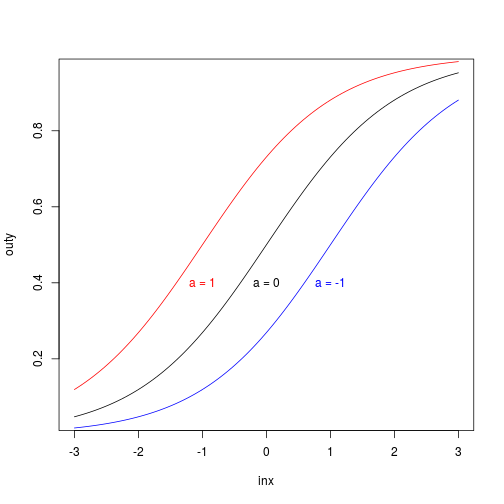
\includegraphics{figure/logitplots1-1.png}
\caption{Changing the value of \(a\)}
\end{figure}

Here's another set of graphs where we change the values of \(b\), or the
coefficient.

\begin{figure}[htbp]
\centering
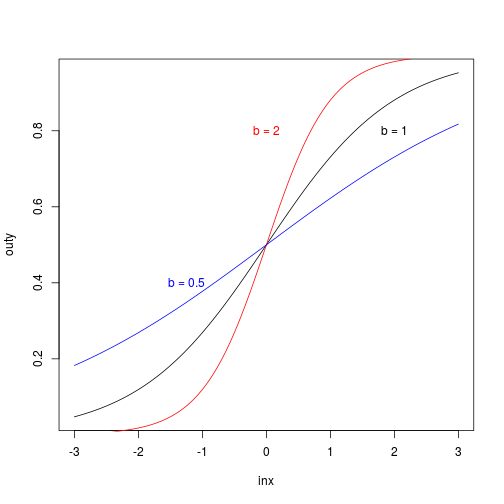
\includegraphics{figure/logitplots2-1.png}
\caption{Changing the value of \(b\)}
\end{figure}

You can see how the higher the value of \(b\), the steeper the curve
becomes. When \(b\) is close to zero, the curve is almost a straight
line.

Of course, \(b\) doesn't need to be positive -- it could be negative.
Here the line would look quite different. As before, the bigger the
magnitude of \(b\), the steeper the line -- though now in the opposite
direction.

Just as in the case of linear regression, we'll ask our software to find
the best fitting values of \(a\) and \(b\).

How can we use this in practice? I'm going to use some data from an
article which, to the best of my knowledge, is the first article to use
random assignment of judges to cases to identify judge effects. The
paper is

Gaudet, Frederk, Harris, Georgeg S., and St.~John, Charles W.,
``Individual differences in the sentencing tendencies of judges'',
published in the journal of the American Institute of Criminal Law and
Criminology in 1933.

Here's a nice paragraph from the article which describes the logic of
investigating judge effects through random assignment:

``Since the rule is that there is no selection of the cases which the
judge is to sentence, but that teh sentencing of a particular prisoner
by a particular judge is a matter of chance (the judges rotate), it is
obvious that, by chance, each judge should get an equal number of cases
whose sentences would normally be long or short\ldots{} Given a
sufficiently large number of cases, if one finds that the average
severity of the sentences of two judges is appreciably different, one is
justified in saying that the factors which determine this difference in
the sentencing tendencies are to be foudn outside of the circumstances
of the crime and those of the prisoner, and hence probably in the judge
since he is the other factor which is always present''.

Here's the authors' table 1:

\begin{figure}[htbp]
\centering
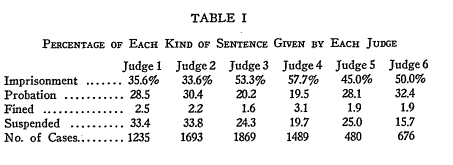
\includegraphics{figure/gaudet_tab1.png}
\caption{Gaudet et al., fig. 1}
\end{figure}

I'm going to concentrate on the decision to imprison.

Here's that information displayed as a graph.

\begin{figure}[htbp]
\centering
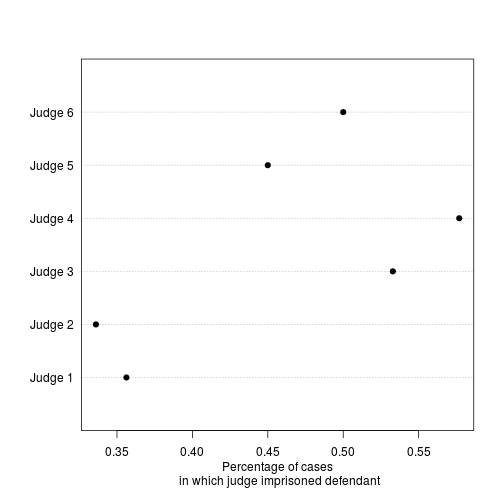
\includegraphics{figure/gaudetplot-1.png}
\caption{plot of chunk gaudetplot}
\end{figure}

What I want to know is: is the difference between Judge 1 and other
judges statistically significant? If we had information on teh whole
population, we wouldn't need to know this. But in this context, we' re
working from a sample, so we can use the mechanism of logistic
regression.

Here's what the data from that article looks like when I've converted it
into the format we need. You can see a column recording the outcome, and
the identity of the judge.

\begin{verbatim}
##        Judge     Sentence
## 1056 Judge 1        Other
## 4801 Judge 4 Imprisonment
## 1853 Judge 2        Other
## 1717 Judge 2 Imprisonment
## 823  Judge 1        Other
## 6486 Judge 5 Imprisonment
\end{verbatim}

Here's how the modelling looks in R.

\begin{Shaded}
\begin{Highlighting}[]
\NormalTok{gaudet_mod <-}\StringTok{ }\KeywordTok{glm}\NormalTok{(}\KeywordTok{I}\NormalTok{(Sentence ==}\StringTok{ "Imprisonment"}\NormalTok{) ~}\StringTok{ }\NormalTok{Judge, }\DataTypeTok{data =} \NormalTok{dat, }\DataTypeTok{family =} \NormalTok{binomial)}
\end{Highlighting}
\end{Shaded}

Here's the output from R

\begin{verbatim}
## 
## Call:
## glm(formula = I(Sentence == "Imprisonment") ~ Judge, family = binomial, 
##     data = dat)
## 
## Deviance Residuals: 
##     Min       1Q   Median       3Q      Max  
## -1.3116  -1.0935  -0.9051   1.1220   1.4767  
## 
## Coefficients:
##              Estimate Std. Error z value Pr(>|z|)    
## (Intercept)  -0.59157    0.05942  -9.956  < 2e-16 ***
## JudgeJudge 2 -0.08920    0.07860  -1.135 0.256419    
## JudgeJudge 3  0.72338    0.07537   9.598  < 2e-16 ***
## JudgeJudge 4  0.90162    0.07926  11.376  < 2e-16 ***
## JudgeJudge 5  0.39090    0.10931   3.576 0.000349 ***
## JudgeJudge 6  0.59157    0.09720   6.086 1.16e-09 ***
## ---
## Signif. codes:  0 '***' 0.001 '**' 0.01 '*' 0.05 '.' 0.1 ' ' 1
## 
## (Dispersion parameter for binomial family taken to be 1)
## 
##     Null deviance: 10267.4  on 7441  degrees of freedom
## Residual deviance:  9979.7  on 7436  degrees of freedom
## AIC: 9991.7
## 
## Number of Fisher Scoring iterations: 4
\end{verbatim}

And here's what it would look like in a published journal article.

\begin{verbatim}
## Error in dimnames(x$coefficients)[[3]]: subscript out of bounds
\end{verbatim}

\begin{verbatim}
## Error in if (tail(stdout, 1) == "") {: argument is of length zero
\end{verbatim}

What does this mean? Let's start from Judge 3.

The coefficient for Judge 3 is 0.72. That means that, compared to Judge
1, Judge 3 is \(e^{0.72}\) = 2.0544332 times more likely to imprison
someone. And because the standard error of this estimate is small
compared to the value of the coefficient, then we know this effect is
likely to exist in the broader population.

\section{Random assignment, multiple
judges}\label{random-assignment-multiple-judges}

The two examples so far have been fairly simplistic. In the first
example, we just used made up data so that we could use an easy model.
In the second example, we used real world data, but we didn't learn
anything about the judge effects that we couldn't have learned just from
looking at the graph. We did learn something about the likely presence
of those effects in the full population. But that might not be that
interesting where we have information on thousands of cases.

I'll therefore move on to some more recent data. This is data from a
book by Cass Sunstein and others. The book is titled, ``Are Judges
Political?''. It's about judges in the US, and so, without wishing to
spoil the ending for you, the answer to the question is, yes: they are.

What Sunstein and his colleagues do is they go through the decisions of
the US federal district courts of appeal. They analyze almost seven
thousand decisions over the period 1995 to 2004. They look at decisions
in aroudn twenty issue areas. For each issue area, they identify what
would be a stereotypical ``liberal'' vote. So, in abortion cases, a
``liberal'' vote is a vote which permits abortion, or strikes down
restrictions on abortion. In a death penalty case, a ``liberal vote'' is
one which restricts the use of the death penalty, and so on.

The unit of analysis in the book is the decision of each individual
judge. Here's an example of some rows of their data.

These are for cases in the 7th circuit, in cases involving the Americans
with disabilities Act.

You can see that some of the variable names are self-explanatory.
Conserve\_vote is obviously conservative vote. Party\_pres isn't
self-explanatory, but I can say that this is a dummy variable which has
value one if the appointing president is a Democrat.

Here's a graph of this same subset of data:

\begin{figure}[htbp]
\centering
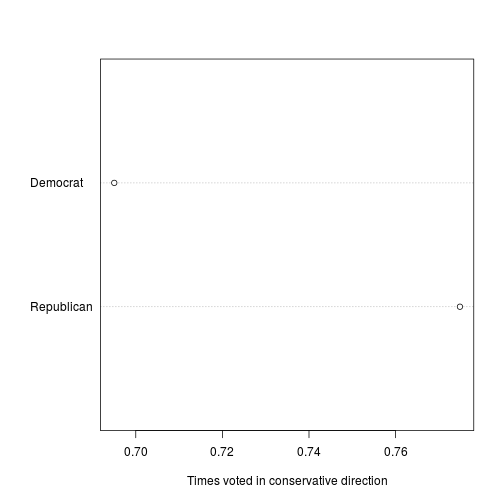
\includegraphics{figure/adaplot-1.png}
\caption{plot of chunk adaplot}
\end{figure}

Now, we can run an analysis of this data. Here's some R code:

\begin{Shaded}
\begin{Highlighting}[]
\NormalTok{mod <-}\StringTok{ }\KeywordTok{glm}\NormalTok{(conserve_vote ~}\StringTok{  }\NormalTok{party_pres, }\DataTypeTok{data=} \NormalTok{dat)}
\end{Highlighting}
\end{Shaded}

And here's the output of that model in R:

\begin{verbatim}
## 
## Call:
## glm(formula = conserve_vote ~ party_pres, data = dat)
## 
## Deviance Residuals: 
##     Min       1Q   Median       3Q      Max  
## -0.7749   0.2251   0.2251   0.2251   0.3050  
## 
## Coefficients:
##             Estimate Std. Error t value Pr(>|t|)    
## (Intercept)  0.77485    0.02333  33.210   <2e-16 ***
## party_pres  -0.07982    0.04318  -1.848   0.0652 .  
## ---
## Signif. codes:  0 '***' 0.001 '**' 0.01 '*' 0.05 '.' 0.1 ' ' 1
## 
## (Dispersion parameter for gaussian family taken to be 0.1861752)
## 
##     Null deviance: 90.186  on 482  degrees of freedom
## Residual deviance: 89.550  on 481  degrees of freedom
## AIC: 562.74
## 
## Number of Fisher Scoring iterations: 2
\end{verbatim}

\begin{verbatim}
## Error in dimnames(x$coefficients)[[3]]: subscript out of bounds
\end{verbatim}

\begin{verbatim}
## Error in if (tail(stdout, 1) == "") {: argument is of length zero
\end{verbatim}

As you can see, it's almost significant, but not quite.

So we can almost say that, compared to Republican judges, Democratic
judges are \(e^{-0.08} = 0.9231163\) times more likely to vote in a
conservative direction.

How can we be sure that this is really the effect of being assigned a
Democratic judge, rather than the kinds of cases Democratic judges hear?
Maybe the Democrats serving on this cicuit at this point in time were
older, more experienced, and heard cases in the balance, cases where
there was a good chance the plaintiff would win?

Well, we can rule that out, because if that was the case, then the
assignment of judges to cases wouldn't be random.

Where the problem comes is when we try and extend this to looking at
different circuits.

The problem here is that although judges are assigned randomly within
circuits, they're not assigned randomly between circuits. As a result,
the chances of a Democratic judge being assigned to a case are very
different depending on which circuit you're in. The 7th circuit, the one
that I just showed you, that's the circuit which is most populated by
Republican appointees. The 9th circuit, by contrast, is the circuit
which is most Democratic. As a result, any differences we find when
comparing across circuits might not be beacuse Democrats are more likely
to vote in a liberal direction, but because circuits with more Democrats
get cases that are more likely to be decided in a liberal direction.

So what can we do? We can start including variables which control for
these effects. In particular, we can include dummy variables for each
circuit.

Here's a short table of the number of votes from each circuit, just
looking again at cases involving ADA claims.

\begin{longtable}[c]{@{}cccccccccccc@{}}
\toprule
\begin{minipage}[b]{0.04\columnwidth}\centering\strut
1
\strut\end{minipage} &
\begin{minipage}[b]{0.04\columnwidth}\centering\strut
2
\strut\end{minipage} &
\begin{minipage}[b]{0.04\columnwidth}\centering\strut
3
\strut\end{minipage} &
\begin{minipage}[b]{0.04\columnwidth}\centering\strut
4
\strut\end{minipage} &
\begin{minipage}[b]{0.04\columnwidth}\centering\strut
5
\strut\end{minipage} &
\begin{minipage}[b]{0.04\columnwidth}\centering\strut
6
\strut\end{minipage} &
\begin{minipage}[b]{0.04\columnwidth}\centering\strut
7
\strut\end{minipage} &
\begin{minipage}[b]{0.04\columnwidth}\centering\strut
8
\strut\end{minipage} &
\begin{minipage}[b]{0.04\columnwidth}\centering\strut
9
\strut\end{minipage} &
\begin{minipage}[b]{0.05\columnwidth}\centering\strut
10
\strut\end{minipage} &
\begin{minipage}[b]{0.05\columnwidth}\centering\strut
11
\strut\end{minipage} &
\begin{minipage}[b]{0.05\columnwidth}\centering\strut
12
\strut\end{minipage}\tabularnewline
\midrule
\endhead
\begin{minipage}[t]{0.04\columnwidth}\centering\strut
236
\strut\end{minipage} &
\begin{minipage}[t]{0.04\columnwidth}\centering\strut
209
\strut\end{minipage} &
\begin{minipage}[t]{0.04\columnwidth}\centering\strut
154
\strut\end{minipage} &
\begin{minipage}[t]{0.04\columnwidth}\centering\strut
89
\strut\end{minipage} &
\begin{minipage}[t]{0.04\columnwidth}\centering\strut
215
\strut\end{minipage} &
\begin{minipage}[t]{0.04\columnwidth}\centering\strut
215
\strut\end{minipage} &
\begin{minipage}[t]{0.04\columnwidth}\centering\strut
483
\strut\end{minipage} &
\begin{minipage}[t]{0.04\columnwidth}\centering\strut
475
\strut\end{minipage} &
\begin{minipage}[t]{0.04\columnwidth}\centering\strut
381
\strut\end{minipage} &
\begin{minipage}[t]{0.05\columnwidth}\centering\strut
259
\strut\end{minipage} &
\begin{minipage}[t]{0.05\columnwidth}\centering\strut
196
\strut\end{minipage} &
\begin{minipage}[t]{0.05\columnwidth}\centering\strut
48
\strut\end{minipage}\tabularnewline
\bottomrule
\end{longtable}

And now here's how our model looks in R:

\begin{Shaded}
\begin{Highlighting}[]
\NormalTok{mod <-}\StringTok{ }\KeywordTok{glm}\NormalTok{(conserve_vote ~}\StringTok{ }\NormalTok{party_pres +}\StringTok{ }\KeywordTok{factor}\NormalTok{(circuit),}
           \DataTypeTok{data =} \NormalTok{ada)}
\end{Highlighting}
\end{Shaded}

and here's what our model would look like in a finished article:

\begin{verbatim}
## Error in dimnames(x$coefficients)[[3]]: subscript out of bounds
\end{verbatim}

\begin{verbatim}
## Error in if (tail(stdout, 1) == "") {: argument is of length zero
\end{verbatim}

Now, what are we to make of this model? First, the coefficient on the
party of the appointing president has changed. Before it was -0.08; now
it's -0.11. So there's been a change in magnitude. Maybe the Democrats
in the 7th circuit are less ideological.

There's also been a change in the statisitsical significance. We're now
very confident that this effect, which exists in the sample, would also
be found in teh population. In part, that's just because of the sample
size. It is easier to get a statistically significant result if you have
lots of data.

This analysis has just looked at one particular type of case: those
involving ADA claims. Of course, we could look at all sorts of different
claims. We would have to include controls for these different areas,
because cases of different types might be more common in different
circuits. But again, once we've controlled for these things, we should
be able to claim that the chances of any given case being heard by a
Democrat are all equal.

\subsection{But was it really random?}\label{but-was-it-really-random}

There's one big assumption that we've been making throughout. We' ve
been happy to assume that cases are randomly assigned to judges. But is
that really the case?

Well, there's been some great detective work on this subject by Matt
Hall. In his paper, ``Randomness reconsidered'', he tries to work out
whether judges really are randomly assigned to cases. What he tries to
do is to run things almost in reverse. Instead of trying to predict the
judge vote using the party of the judge, he uses features of the case to
try and predict the party of the judge. If judges are really randomly
assigned to cases, then this won't be possible. There just won't be any
way to predict the party of the judge hearing the case.

But what he finds is that there are significant effects. The odds of
Democratic judges hearing certain cases are slightly different.

And so he went back, and tried to work out why that was the case:

He found two main reasons.

First, although Sunstein et al controlled for the circuit, circuit
compositions change over time. In this period, circuits could become
either more Democratic, or more Republican. Although at any single point
in time, cases are randomly allocated, over the period of ten years
cases at certain points might have better odds of getting heard by a
Democrat. If those over time changes coincide with changes in teh
winnability of cases, it'll mess up our analysis.

Second, there were some circuits which just didn't practice
randomization. How did Hall find this out? He called up the clerks in
these circuits. He found that ``random assignment was not used in the
Fourth Circuit before the year 2000,the Fifth and Eighth Circuits before
2003, or the Tenth Circuit before 1998''.

Now, the main finding of the book doesn't change. Judges still vote
politically. But when you account for tehse slight differences, the size
of the effect changes. In fact, it gets slightly bigger.

\section{Random assignment, multiple judges, aggregate
outcome}\label{random-assignment-multiple-judges-aggregate-outcome}

The analysis presented by Sunstein is a bit funny. Normally, when we
think of random assignment, we think of it as a way of investigating
effects on things that are treated. A treatment is randomly assigned to
a test subject, and something happens to the test subject.

In the Sunstein case, a judge is randomly assigned to a case, but
instead of looking at what happens to the case, we look at what happens
to the judge's vote. That feels strange.

It would be more normal to investigate what's happening to the case
level outcome. After all, it's the judges that are being assigned to the
case. Why can't we predict the case outcome, using the assignment of
judges.

There are a couple of problems with this.

Let's suppose I have a case before a court.

Let's suppose that two judges have already been randomly assigned to the
case.

One of these judges is conservative, and one is liberal.

Now we randomly choose a final, third judge.

Let's just assume that, if the third judge is conservative, the two
conservative judges vote together. And if the third judge is liberal,
two liberal judges vote together.

If all the cases were like this, then we'd be able to identify a nice
effect.

But now, let's change the default setup.

Let's start with two conservative judges. That's a majority of the
court. And so if we add a conservative judge, we don't get any change.
And if we add a liberal judge, we don't get any change. But by
constrsuction, we set it up so that liberal judges would vote liberally,
and conservative judges conservatively. If we only looked at cases like
this, we'd never recover that effect.

If we had some cases of teh first type, and some cases of the second
type, we'd recover some effect, but it would be attenuated by the cases
of the second type.

And so, if you want to examine case outcomes, you have to be smart.

You can restrict your comparisons. You can compare cases which have DDR
to DDD, and identify that effect. You can compare cases which have RRD
to RRR, and identify that effect. You can compare cases which have DRD
to DRR, and identify that effect. But you'll never identify the effect
of adding an extra D or an extra R per se.

Or you can get more complicated. There's a paper by Ben Lauderdale,
Dominik Hangartner, and Judith Spirig, which sets up different
aggregation mechanisms: either the median judge decides, or the
rapporteur decides, or the panel's decision is a mean of the different
judge's positions, and so on. The problem is that in order to apply
these different aggregation rules, they have to use fairly complicated
statistics. In particular, they use Bayesian statistics, and posit an
underlying position associated with each judge. Those underlying
positions are modelled using other regression variables, and aggregated
using a particular mechanism. They look at which mechanisms best fit the
data, and they're able to talk about the effects of being appointed by a
particular party on the scale of the latent dimension.

That approach -- of positing different unknown things -- also fetaures
in the stuff that comes across the break. So let's pause there for a
moment, and resume after the break, when we'll be discussing item
respones moedls.

\section{Ideal point analysis:
insight}\label{ideal-point-analysis-insight}

The previous section was concerned with analyzing differences between
cases. In this section, we turn to looking at differences within cases.
That is, we turn to the analysis of dissent.

Obviously not every court allows dissent. In such cases, you may need to
use one of the more complicated models discussed in the previous
section. There are good papers which have been written on this. In
addition to the paper by Lauderdale et al., there's a paper by Michael
Malecki, which looks at the European Court of Justice.

In a moment, I'm going to discuss a particular model for dissenting
votes. But it's important to start simple.

I'm going to start with some of the data from the Supreme Court
Database, sometimes called the Spaeth database. This contains
information on every case decided by the Supreme Court.

Here, I'm focusing just on cases from 2010 onwards. That makes things a
bit more manageable

I've had to put in a bit of work into reshaping the data. The SCDB
records information in a ``long'' format. Each row corresponds to a
judge-case combination. I've reshaped that so that it's in a wide
format. Here, each row corresponds to a case, and there are lots of
columns for each judge. Here are the first couple of rows

\begin{longtable}[c]{@{}ccccccc@{}}
\caption{Table continues below}\tabularnewline
\toprule
\begin{minipage}[b]{0.10\columnwidth}\centering\strut
caseId
\strut\end{minipage} &
\begin{minipage}[b]{0.13\columnwidth}\centering\strut
AMKennedy
\strut\end{minipage} &
\begin{minipage}[b]{0.11\columnwidth}\centering\strut
AScalia
\strut\end{minipage} &
\begin{minipage}[b]{0.11\columnwidth}\centering\strut
CThomas
\strut\end{minipage} &
\begin{minipage}[b]{0.10\columnwidth}\centering\strut
EKagan
\strut\end{minipage} &
\begin{minipage}[b]{0.13\columnwidth}\centering\strut
JGRoberts
\strut\end{minipage} &
\begin{minipage}[b]{0.13\columnwidth}\centering\strut
RBGinsburg
\strut\end{minipage}\tabularnewline
\midrule
\endfirsthead
\toprule
\begin{minipage}[b]{0.10\columnwidth}\centering\strut
caseId
\strut\end{minipage} &
\begin{minipage}[b]{0.13\columnwidth}\centering\strut
AMKennedy
\strut\end{minipage} &
\begin{minipage}[b]{0.11\columnwidth}\centering\strut
AScalia
\strut\end{minipage} &
\begin{minipage}[b]{0.11\columnwidth}\centering\strut
CThomas
\strut\end{minipage} &
\begin{minipage}[b]{0.10\columnwidth}\centering\strut
EKagan
\strut\end{minipage} &
\begin{minipage}[b]{0.13\columnwidth}\centering\strut
JGRoberts
\strut\end{minipage} &
\begin{minipage}[b]{0.13\columnwidth}\centering\strut
RBGinsburg
\strut\end{minipage}\tabularnewline
\midrule
\endhead
\begin{minipage}[t]{0.10\columnwidth}\centering\strut
2010-001
\strut\end{minipage} &
\begin{minipage}[t]{0.13\columnwidth}\centering\strut
1
\strut\end{minipage} &
\begin{minipage}[t]{0.11\columnwidth}\centering\strut
1
\strut\end{minipage} &
\begin{minipage}[t]{0.11\columnwidth}\centering\strut
1
\strut\end{minipage} &
\begin{minipage}[t]{0.10\columnwidth}\centering\strut
1
\strut\end{minipage} &
\begin{minipage}[t]{0.13\columnwidth}\centering\strut
1
\strut\end{minipage} &
\begin{minipage}[t]{0.13\columnwidth}\centering\strut
1
\strut\end{minipage}\tabularnewline
\begin{minipage}[t]{0.10\columnwidth}\centering\strut
2010-002
\strut\end{minipage} &
\begin{minipage}[t]{0.13\columnwidth}\centering\strut
1
\strut\end{minipage} &
\begin{minipage}[t]{0.11\columnwidth}\centering\strut
1
\strut\end{minipage} &
\begin{minipage}[t]{0.11\columnwidth}\centering\strut
1
\strut\end{minipage} &
\begin{minipage}[t]{0.10\columnwidth}\centering\strut
1
\strut\end{minipage} &
\begin{minipage}[t]{0.13\columnwidth}\centering\strut
1
\strut\end{minipage} &
\begin{minipage}[t]{0.13\columnwidth}\centering\strut
1
\strut\end{minipage}\tabularnewline
\begin{minipage}[t]{0.10\columnwidth}\centering\strut
2010-003
\strut\end{minipage} &
\begin{minipage}[t]{0.13\columnwidth}\centering\strut
1
\strut\end{minipage} &
\begin{minipage}[t]{0.11\columnwidth}\centering\strut
1
\strut\end{minipage} &
\begin{minipage}[t]{0.11\columnwidth}\centering\strut
1
\strut\end{minipage} &
\begin{minipage}[t]{0.10\columnwidth}\centering\strut
1
\strut\end{minipage} &
\begin{minipage}[t]{0.13\columnwidth}\centering\strut
1
\strut\end{minipage} &
\begin{minipage}[t]{0.13\columnwidth}\centering\strut
1
\strut\end{minipage}\tabularnewline
\begin{minipage}[t]{0.10\columnwidth}\centering\strut
2010-004
\strut\end{minipage} &
\begin{minipage}[t]{0.13\columnwidth}\centering\strut
1
\strut\end{minipage} &
\begin{minipage}[t]{0.11\columnwidth}\centering\strut
1
\strut\end{minipage} &
\begin{minipage}[t]{0.11\columnwidth}\centering\strut
1
\strut\end{minipage} &
\begin{minipage}[t]{0.10\columnwidth}\centering\strut
1
\strut\end{minipage} &
\begin{minipage}[t]{0.13\columnwidth}\centering\strut
1
\strut\end{minipage} &
\begin{minipage}[t]{0.13\columnwidth}\centering\strut
1
\strut\end{minipage}\tabularnewline
\bottomrule
\end{longtable}

\begin{longtable}[c]{@{}ccc@{}}
\toprule
\begin{minipage}[b]{0.13\columnwidth}\centering\strut
SAAlito
\strut\end{minipage} &
\begin{minipage}[b]{0.14\columnwidth}\centering\strut
SGBreyer
\strut\end{minipage} &
\begin{minipage}[b]{0.15\columnwidth}\centering\strut
SSotomayor
\strut\end{minipage}\tabularnewline
\midrule
\endhead
\begin{minipage}[t]{0.13\columnwidth}\centering\strut
1
\strut\end{minipage} &
\begin{minipage}[t]{0.14\columnwidth}\centering\strut
1
\strut\end{minipage} &
\begin{minipage}[t]{0.15\columnwidth}\centering\strut
1
\strut\end{minipage}\tabularnewline
\begin{minipage}[t]{0.13\columnwidth}\centering\strut
1
\strut\end{minipage} &
\begin{minipage}[t]{0.14\columnwidth}\centering\strut
1
\strut\end{minipage} &
\begin{minipage}[t]{0.15\columnwidth}\centering\strut
1
\strut\end{minipage}\tabularnewline
\begin{minipage}[t]{0.13\columnwidth}\centering\strut
1
\strut\end{minipage} &
\begin{minipage}[t]{0.14\columnwidth}\centering\strut
1
\strut\end{minipage} &
\begin{minipage}[t]{0.15\columnwidth}\centering\strut
1
\strut\end{minipage}\tabularnewline
\begin{minipage}[t]{0.13\columnwidth}\centering\strut
1
\strut\end{minipage} &
\begin{minipage}[t]{0.14\columnwidth}\centering\strut
1
\strut\end{minipage} &
\begin{minipage}[t]{0.15\columnwidth}\centering\strut
1
\strut\end{minipage}\tabularnewline
\bottomrule
\end{longtable}

With the information in this format, we can calculate some simple
statistics. For example, the average rate of agreement between two
judges on SCOTUS is 75. The lowest rate of agreement is 59; that's
between RBGinsburg and CThomas.

Those figures are calculated on the basis of 387 cases. Now, if the
figure had been based on a tiny handful of cases, we might think it
possible for these two judges to disagree at this rate just by chance.
Maybe they really agree at the average rate, they just got unlucky.

We can test this by calculating the 95\% confidence interval for this
proportion. There are a number of online calculators for this. I'll just
show you how I'd do it in R.

\begin{Shaded}
\begin{Highlighting}[]
\NormalTok{times.judges.agreed <-}\StringTok{ }\DecValTok{228}
\NormalTok{times.judges.sat.together <-}\StringTok{ }\DecValTok{387}
\KeywordTok{binom.test}\NormalTok{(times.judges.agreed,}
           \NormalTok{times.judges.sat.together,}
           \DataTypeTok{p =} \FloatTok{0.75}\NormalTok{)}
\end{Highlighting}
\end{Shaded}

\begin{verbatim}
## 
##  Exact binomial test
## 
## data:  times.judges.agreed and times.judges.sat.together
## number of successes = 228, number of trials = 387, p-value =
## 5.261e-12
## alternative hypothesis: true probability of success is not equal to 0.75
## 95 percent confidence interval:
##  0.5383110 0.6386093
## sample estimates:
## probability of success 
##              0.5891473
\end{verbatim}

Let's now switch to a different example. I've also got data on judges'
dissents on the UK Supreme Court. The UK Supreme Court is a bit
different, because not all judges sit on all cases.

But looking just at the judges currently serving on the court, it's
interesting to compare LAdy Hale and Lord Sumption. These two judges are
often supposed to have very different political viewpoints. They've sat
together in 26 cases. They've agreed in 81 percent of those, or 21.
That's lower than the general rate of agreement on the court, which is
84\%.

So what's the probability that these two could have a rate of agreement
which is actually 84\%, but which in fact is much higher? We can
calculate the same confidence intervals.

\begin{Shaded}
\begin{Highlighting}[]
\NormalTok{times.judges.agreed <-}\StringTok{ }\DecValTok{21}
\NormalTok{times.judges.sat.together <-}\StringTok{ }\DecValTok{26}
\KeywordTok{binom.test}\NormalTok{(times.judges.agreed,}
           \NormalTok{times.judges.sat.together,}
           \DataTypeTok{p =} \FloatTok{0.84}\NormalTok{)}
\end{Highlighting}
\end{Shaded}

\begin{verbatim}
## 
##  Exact binomial test
## 
## data:  times.judges.agreed and times.judges.sat.together
## number of successes = 21, number of trials = 26, p-value = 0.5954
## alternative hypothesis: true probability of success is not equal to 0.84
## 95 percent confidence interval:
##  0.6064945 0.9344519
## sample estimates:
## probability of success 
##              0.8076923
\end{verbatim}

So before you do any kind of advanced analysis, take care to look just
at the raw rates of agreement between judges. If those don't show any
clear patterns -- if judges who are supposed to be political opposites
don't display rates of agreement that are significantly lower than
others -- well, then you might want to abandon this kind of research.

Now, it's possible to carry on with this kind of analysis. You can
calculate rates of agreement for each pair of judges. And you can create
a big spreadsheet, and try and reorder judges until judges with higher
rates of agreement are closer to each other.

But that way of proceeding is really unwieldy. If you just take a court
with three judges on it, there are three comparisons to be made. A court
with five judges on it, has 10 comparisons to be made. A court with nine
judges? 36 comparisons. That's a lot of comparisons to make. And there's
no guarantee that we'll be able to make sense of those comparisons, or
use them to arrange judges in a simple order.

Ideal point analysis is a solution to this problem. There are a number
of assumptions to make in ideal point analysis, so I'll start
restrictively and work through them.

The first thing I'll need is some notation.

I'll need some indices. First, I'll need to talk about judges, so I'll
use \(j\) to refer to judges, and these judges will be numbered from
one, up to arbitrary number \(J\). Second, I'll need to talk about
cases, so I'll use \(i\) to refer to cases, and these cases will be
numbered in a similar way.

With those two indices at hand, I can now talk about the vote of each
judge in each case. I'll call that \(y_{ij}\). That's the outcome;
that's the thing to be explained. I'm going to say that this variable
can either be a one or a zero.

In this exposition, we'll start by saying

I'll start by introducing some notation.

I'm going to need to refer to judges, and so I'll use \(j\) to stand for
the judge that I'm talking about at any particular time. \(j\) will
start at 1, for Judge 1, and run up to \(J\).

I'll also need to refer to cases, and so I'll use \(i\) to refer to
cases. \(i\) will be numbered in the same way, running up to \(I\).

I'm now going to ask you to believe in certain properties of judges,
properties which can't be empirically verified, but which are used in
the model. In particular, I'm going to ask you to believe that each
judge has something called an \emph{ideal point} in space. Because we're
keeping it simple, that space is just going to be one-dimensional.
Judges' ideal points are just points on the number line. One judge could
have an ideal point of minus two, another judge could have an ideal
point of plus three, and so on.

In very many analysis of judicial behaviour, that one-dimensional space
is assumed to be a political dimension, which runs from left to right.
Typically, higher numbers correspond to more right-wing positions,
because number lines go from smaller numbers on the left to bigger
numbers on the right.

I'm going to use the Greek character \(\theta\) to refer to this ideal
point. I'm going to subscript \(\theta\) using \(j\), to show that it's
a property of judges.

I'm now going to ask you to believe in certain properties of cases. I'm
going to ask you to believe that each case has a location in this same
space in which we find our judges. You can call this the case's
location, or if you're old fashioned, you can talk about the case
cutpoint.

The case location doesn't have an easy interpretation. It's really
defined in terms of the outcome. The case location is supposed to divide
judges on one side of the cutpoint -- who vote one way -- from judges on
the other side of the cutpoint, who vote a different way. Judges who
have an ideal point exactly equal to the case location are supposed to
be indifferent. The characterisation of the cut-point will become
clearer when we try to link it to the vote.

I'm going to use \(\alpha\) to refer to the case location. And I'm going
to subscript it using \(i\), to show that it's a property of cases.

So let's talk about the vote. I'll use \(y_{ij}\) to refer to the vote,
in case \(i\), of judge \(j\). By convention, I'll say that this
variable has the value of one when the judge votes with the majority,
and has the value of zero when the judge dissents. This decision doesn't
have any consequences. We could code judges' decisions in the opposite
way, and it wouldn't affect our findings.

Now, for the purpose of exposition, I'm going to introduce an assumption
which I'll relax later. I'm going to assume that this is a court with a
conservative majority, which generally reaches conservative decisions.
If that's so, then the cutpoint will split the majority, on the right,
from a minority, on the left.

With that assumption in place, I can sketch out a relationship between

\begin{itemize}
\tightlist
\item
  a judge's ideal point, and
\item
  a judge's vote in a particular case.
\end{itemize}

Here's that relationship visually. As we move from left to right, the
probability of casting a vote for the majority grows. When we reach the
case location, the probability of casting a vote for the majority is
50:50. As we move further to the right, the probability of casting a
vote for the majority increases to one.

Now, that curve should look familiar to you from the first half of the
session. It's the logistic curve. We can describe that curve using the
same equation as before:

\[
p = \frac{1}{1 + e^{-a + bx}}
\]

I'm going to replace two of the letters in that equation by the
specialised terms we used before, and scrub out the b.

\[
p = \frac{1}{1 + e^{-\alpha_i + \theta_j}}
\]

Alternately,

\[
p = \frac{1}{1 + e^{\theta_j-\alpha_i}}
\]

So you subtract the case location parameter from the ideal point, and if
you're still left with a positive number, they're more likely to vote
with the majority, and vice versa.

So if you know that voting with the majority is always going to be
voting in a conservative direction, and if you know that each case is
equally important with respect to this pattern of left-right voting,
then you can stop there. But of course, we don't know that. There might
be cases which don't matter at all for ideological voting.

How could we represent those? Well, here I'm going to reintroduce a
character I deleted earlier, the b. I'm going to call this the case
discrimination parameter. Essentially, it's going to model how
responsive judges votes are to their distance from the case location. If
the b is very large in magnitude, then this case is going to be very
good at splitting judges. If the b is very low in magnitude, it'll be
very poor at splitting judges.

Here are two possible values of b. In the first case, the value of b is
very high, and we model the probability of judges voting with the
majority as rising very quickly with their difference from the case
location. In the second case, the value of b is very low, almost flat.
You might think of this case as a procedural case.

So introducing \(b\) helps us with cases which seem less political, or
which, in technical terms, discriminate less well with respect to the
recovered dimension. But \(b\) also helps us with the possibility that
sometimes, you might have majorities of different political complexions.

Here, for example, is a case with negative \(b\). In this instance, it's
judges to the right who are less likely to vote with the majority. The
line slopes down.

And this is the magic of ideal point analysis. We can carry out our
analysis without having to consider the ideological character of the
majority outcome.

At this point, we've been able to provide equations to model how judges
vote. Our general strategy will be to estimate possible values of
\(\theta\), \(\alpha\), \(\beta\), and so on, so as to best explain the
observed voting patterns. If we predict a judge will vote with the
majority, and they instead vote with the minority, we can adjust their
ideal point a little. Or we can adjust the case location. Or we can
adjust the case discrimination parameter.

In fact, we're in danger of becoming a bit too flexible. As it stands,
our model is unidentified. That means that we can change the parameters
without affecting how well it explains the data.

Two examples:

\begin{itemize}
\tightlist
\item
  we could multiply all the judge ideal points and the discrimination
  parameters by minus one (flipping)
\item
  we could divide all the judge ideal points and the discrimination
  parameters by some constant (shrinking/expanding)
\end{itemize}

We need to fix some things in order to get some numbers out. In most
applications, it's common to fix the locations of two judges. Take one
judge who is rumoured to be on the left, and set their value of
\(\theta\) to -1. Take one judge who is rumoured to be on the right, and
set their value of \(\theta\) to +1.

That allows us to determine both the scale of the numbers, and the
direction.

So with these constraints in place, we can get the computer to estimate
the best set of numbers to explain the data we have. This process, even
with these constraints, is quite computationally demanding. I'll not
discuss how the estimation works here, but it cannot often run
overnight. So if you're running some of the code below, don't expect it
to finish in a couple of minutes!

How does this work in practice?

Well, there are two software packages I know of which make ideal point
estimation relatively easy.

The first of these is a package called MCMCpack, which estimates a
variety of models. MCMCpack uses Bayesian methods, like almost all
applications of ideal point analysis. And it does so using Markov Chain
Monte Carlo, hence the name of the package. Within the MCMCpack package,
there's a function, MCMCirt1d, which estimates one-dimensional item
response models. That's just another name for ideal point analysis.

The second package, and the package which I would probably recommend, is
pscl. That stands for political science computation laboratory. It's
written by Simon Jackman, who's an expert on Bayesian analysis, and it
includes a function, ideal, to estimate ideal points.

Key to both packages is getting your data in the right format. MCMCpack
will take an ordinary array or data frame in R. PSCL requires the data
to be in its own format.

Let me remind you of some of the data we have to deal with:

\begin{longtable}[c]{@{}ccccccc@{}}
\caption{Table continues below}\tabularnewline
\toprule
\begin{minipage}[b]{0.10\columnwidth}\centering\strut
caseId
\strut\end{minipage} &
\begin{minipage}[b]{0.13\columnwidth}\centering\strut
AMKennedy
\strut\end{minipage} &
\begin{minipage}[b]{0.11\columnwidth}\centering\strut
AScalia
\strut\end{minipage} &
\begin{minipage}[b]{0.11\columnwidth}\centering\strut
CThomas
\strut\end{minipage} &
\begin{minipage}[b]{0.10\columnwidth}\centering\strut
EKagan
\strut\end{minipage} &
\begin{minipage}[b]{0.13\columnwidth}\centering\strut
JGRoberts
\strut\end{minipage} &
\begin{minipage}[b]{0.13\columnwidth}\centering\strut
RBGinsburg
\strut\end{minipage}\tabularnewline
\midrule
\endfirsthead
\toprule
\begin{minipage}[b]{0.10\columnwidth}\centering\strut
caseId
\strut\end{minipage} &
\begin{minipage}[b]{0.13\columnwidth}\centering\strut
AMKennedy
\strut\end{minipage} &
\begin{minipage}[b]{0.11\columnwidth}\centering\strut
AScalia
\strut\end{minipage} &
\begin{minipage}[b]{0.11\columnwidth}\centering\strut
CThomas
\strut\end{minipage} &
\begin{minipage}[b]{0.10\columnwidth}\centering\strut
EKagan
\strut\end{minipage} &
\begin{minipage}[b]{0.13\columnwidth}\centering\strut
JGRoberts
\strut\end{minipage} &
\begin{minipage}[b]{0.13\columnwidth}\centering\strut
RBGinsburg
\strut\end{minipage}\tabularnewline
\midrule
\endhead
\begin{minipage}[t]{0.10\columnwidth}\centering\strut
2010-001
\strut\end{minipage} &
\begin{minipage}[t]{0.13\columnwidth}\centering\strut
1
\strut\end{minipage} &
\begin{minipage}[t]{0.11\columnwidth}\centering\strut
1
\strut\end{minipage} &
\begin{minipage}[t]{0.11\columnwidth}\centering\strut
1
\strut\end{minipage} &
\begin{minipage}[t]{0.10\columnwidth}\centering\strut
1
\strut\end{minipage} &
\begin{minipage}[t]{0.13\columnwidth}\centering\strut
1
\strut\end{minipage} &
\begin{minipage}[t]{0.13\columnwidth}\centering\strut
1
\strut\end{minipage}\tabularnewline
\begin{minipage}[t]{0.10\columnwidth}\centering\strut
2010-002
\strut\end{minipage} &
\begin{minipage}[t]{0.13\columnwidth}\centering\strut
1
\strut\end{minipage} &
\begin{minipage}[t]{0.11\columnwidth}\centering\strut
1
\strut\end{minipage} &
\begin{minipage}[t]{0.11\columnwidth}\centering\strut
1
\strut\end{minipage} &
\begin{minipage}[t]{0.10\columnwidth}\centering\strut
1
\strut\end{minipage} &
\begin{minipage}[t]{0.13\columnwidth}\centering\strut
1
\strut\end{minipage} &
\begin{minipage}[t]{0.13\columnwidth}\centering\strut
1
\strut\end{minipage}\tabularnewline
\begin{minipage}[t]{0.10\columnwidth}\centering\strut
2010-003
\strut\end{minipage} &
\begin{minipage}[t]{0.13\columnwidth}\centering\strut
1
\strut\end{minipage} &
\begin{minipage}[t]{0.11\columnwidth}\centering\strut
1
\strut\end{minipage} &
\begin{minipage}[t]{0.11\columnwidth}\centering\strut
1
\strut\end{minipage} &
\begin{minipage}[t]{0.10\columnwidth}\centering\strut
1
\strut\end{minipage} &
\begin{minipage}[t]{0.13\columnwidth}\centering\strut
1
\strut\end{minipage} &
\begin{minipage}[t]{0.13\columnwidth}\centering\strut
1
\strut\end{minipage}\tabularnewline
\begin{minipage}[t]{0.10\columnwidth}\centering\strut
2010-004
\strut\end{minipage} &
\begin{minipage}[t]{0.13\columnwidth}\centering\strut
1
\strut\end{minipage} &
\begin{minipage}[t]{0.11\columnwidth}\centering\strut
1
\strut\end{minipage} &
\begin{minipage}[t]{0.11\columnwidth}\centering\strut
1
\strut\end{minipage} &
\begin{minipage}[t]{0.10\columnwidth}\centering\strut
1
\strut\end{minipage} &
\begin{minipage}[t]{0.13\columnwidth}\centering\strut
1
\strut\end{minipage} &
\begin{minipage}[t]{0.13\columnwidth}\centering\strut
1
\strut\end{minipage}\tabularnewline
\bottomrule
\end{longtable}

\begin{longtable}[c]{@{}ccc@{}}
\toprule
\begin{minipage}[b]{0.13\columnwidth}\centering\strut
SAAlito
\strut\end{minipage} &
\begin{minipage}[b]{0.14\columnwidth}\centering\strut
SGBreyer
\strut\end{minipage} &
\begin{minipage}[b]{0.15\columnwidth}\centering\strut
SSotomayor
\strut\end{minipage}\tabularnewline
\midrule
\endhead
\begin{minipage}[t]{0.13\columnwidth}\centering\strut
1
\strut\end{minipage} &
\begin{minipage}[t]{0.14\columnwidth}\centering\strut
1
\strut\end{minipage} &
\begin{minipage}[t]{0.15\columnwidth}\centering\strut
1
\strut\end{minipage}\tabularnewline
\begin{minipage}[t]{0.13\columnwidth}\centering\strut
1
\strut\end{minipage} &
\begin{minipage}[t]{0.14\columnwidth}\centering\strut
1
\strut\end{minipage} &
\begin{minipage}[t]{0.15\columnwidth}\centering\strut
1
\strut\end{minipage}\tabularnewline
\begin{minipage}[t]{0.13\columnwidth}\centering\strut
1
\strut\end{minipage} &
\begin{minipage}[t]{0.14\columnwidth}\centering\strut
1
\strut\end{minipage} &
\begin{minipage}[t]{0.15\columnwidth}\centering\strut
1
\strut\end{minipage}\tabularnewline
\begin{minipage}[t]{0.13\columnwidth}\centering\strut
1
\strut\end{minipage} &
\begin{minipage}[t]{0.14\columnwidth}\centering\strut
1
\strut\end{minipage} &
\begin{minipage}[t]{0.15\columnwidth}\centering\strut
1
\strut\end{minipage}\tabularnewline
\bottomrule
\end{longtable}

I'm going to have to transform that data in order to get it into our
packages. Here's the R code I would use.

\begin{Shaded}
\begin{Highlighting}[]
\NormalTok{### Get the third column to the last column}
\NormalTok{vote.mat <-}\StringTok{ }\NormalTok{scdb.c[,}\DecValTok{3}\NormalTok{:}\KeywordTok{ncol}\NormalTok{(scdb.c)]}
\NormalTok{### Store the judge names}
\NormalTok{judge.names <-}\StringTok{ }\KeywordTok{names}\NormalTok{(vote.mat)}
\NormalTok{### Convert the data to a matrix}
\NormalTok{vote.mat <-}\StringTok{ }\KeywordTok{as.matrix}\NormalTok{(vote.mat)}
\NormalTok{### Transpose it}
\NormalTok{vote.mat <-}\StringTok{ }\KeywordTok{t}\NormalTok{(vote.mat)}
\NormalTok{### Show the first three judges and}
\NormalTok{### the first ten cases}
\NormalTok{vote.mat[}\DecValTok{1}\NormalTok{:}\DecValTok{3}\NormalTok{,}\DecValTok{1}\NormalTok{:}\DecValTok{10}\NormalTok{]}
\end{Highlighting}
\end{Shaded}

So how would we get that into our analysis?

\begin{Shaded}
\begin{Highlighting}[]
\NormalTok{### Test run}
\NormalTok{model <-}\StringTok{ }\KeywordTok{MCMCpack}\NormalTok{(vote.mat,}
                  \DataTypeTok{theta.constraints =} \KeywordTok{list}\NormalTok{(}\StringTok{"AScalia"} \NormalTok{=}\StringTok{ }\DecValTok{1}\NormalTok{,}
                                           \StringTok{"SSotomayor"} \NormalTok{=}\StringTok{ }\NormalTok{-}\DecValTok{1}\NormalTok{),}
                  \DataTypeTok{burnin=}\DecValTok{50}\NormalTok{,}
                  \DataTypeTok{mcmc=}\DecValTok{100}\NormalTok{,}
                  \DataTypeTok{thin=}\DecValTok{2}\NormalTok{,}
                  \DataTypeTok{verbose=}\DecValTok{5}\NormalTok{,}
                        \DataTypeTok{store.item=}\OtherTok{TRUE}\NormalTok{)}
\end{Highlighting}
\end{Shaded}

\begin{verbatim}
## Error in eval(expr, envir, enclos): could not find function "MCMCpack"
\end{verbatim}

MCMCpack -- rows to subjects pscl -- ibid.

\hypertarget{refs}{}

\end{document}
